% !TEX root =  master.tex
\chapter{Projektphase 1 – Firewall}
Die Firewall-Konfigurationen werden mittels IP-Tables auf der Opfermaschine erstellt. Dabei wurden Bash-Scripts implementiert, um die jeweils notwendigen Befehle nachvollziehen zu können. Zudem wird sämtlicher Datenverkehr der Penetrationstests aufgezeichnet und interpretiert. 
\section{Offene Konfiguration}

Zunächst wird auf der Opfermaschine eine offene Konfiguration der Firewall erstellt. Das bedeutet in diesem Fall, dass jeglicher einkehrender sowie jeglicher auskehrende Datenverkehr ungehindert zugelassen wird. In dieser Konfiguration werden weder Kommunikationsquellen noch Inhalt gefiltert oder geblockt.

\subsection{Script}
Der erste Schritt setzt die IP-Tables auf ihre Ursprungswerte zurück. Das heißt, dass alle einkommenden, ausgehenden und weitergeleiteten Pakete ungefiltert zugelassen werden. Zusätzlich zu der normalen IP-Tables Konfiguration wird hier auch noch die NAT-Konfiguration gesetzt.  
Das Script besteht aus drei wesentlichen Prozessen: 
\begin{itemize}
	\item Einstellung der Regeln (inklusive NAT)
	\item Flushing der Regeln
	\item Logging
\end{itemize} 

Als nächstes werden alle noch überbleibenden Ausnahmeregelungen `geflushed`. Das bedeutet, dass diese gelöscht und auf den Standardwert zurückgesetzt werden. Dies ermöglicht es eine saubere Basiskonfiguration zu erhalten.\\
Abschließend wird das Logging behandelt. Damit am Ende des Vorgangs nachvollzogen werden kann, welche Pakte eingetroffen bzw. ausgetreten sind, wird der Datenverkehr vom Script aus protokolliert.
Zusätzlich zu den drei Funktionen des Scripts wird nach Abschluss die Konfiguration in der Konsole ausgegeben.

\newpage

\lstinputlisting[language=bash]{scripts/firewall-open.sh}

\newpage
Output: 
\lstinputlisting[]{scripts/output_firewall-open.sh}

\subsection{Penetrationtest – Inward}
Da nun die Firewall der Opfermaschine konfiguriert wurde, können Penetrationstests durchgeführt werden. 
Zunächst wird geprüft, welche Informationen über einen Portscan mit NMAP herausgefunden werden können. 
Während der laufenden Scans wird zusätzlich der Datenverkehr der Opfermaschine mit Hilfe von Wireshark aufgezeichnet. 
Dies hilft dabei die Reaktion – bzw. das Fehlen einer Reaktion – der Opfermaschine nachzuvollziehen.
\subsubsection{nmap 10.0.2.4 -p- -A -T4}
Der erste NMAP-Scan wird mit vier paramentern versehen. Zunächst muss die Zieladresse des Opfers angegeben werden. In diesem Fall befindet sich das Opfer im NAT-Netzwerk an der Adresse 10.0.2.4. Als nächstes wird die gewünschte Menge der Ports angegeben. Standardmäßig werden die 1000 wichtigsten Ports geprüft. Auf Grund der Gründlichkeit dieses Tests werden jedoch alle 65.535 Ports der Opfermaschine gescannt – zu erkennen am Parameter -p-. Darauf folgend wird erneut ein Parameter zu Gunsten der Gründlichkeit gesetzt. Der Parameter -A setzt die Aggressivität des Scans. So werden durch diesen Parameter Funktionen wie OS-Detection, Version-Scanning, Script-Scanning und Traceroute verwendet. Zuletzt wird ein Geschwindigkeitsparameter gesetzt. \\

Output:
\lstinputlisting[]{scripts/scans/nmap_p_A_T4}

Im Output ist zu erkennen, dass alle gescannten Ports geschlossen sind. Dies war zu erwarten, da auf der Opfermaschine keine Services laufen und somit keine Ports genutzt werden. Dennoch lässt der Fakt, dass die Ports als geschlossen gezeigt werden, auf weitere Informationen schließen. Zum einen wird dadurch bekannt, dass die Anfragen ungefiltert an die Opfermaschine durchgekommen sind. Im gleichen Zuge wird erkannt, dass die Angreifermaschiene Antworten auf ihre Anfragen erhalten hat. Demnach kann der Angreifer zu dem Entschluss kommen, dass die Firewall offen ist. 
Zusätzlich zu dem Portstatus wird die MAC-Adresse und der Hersteller des Geräts identifiziert. Zudem versucht das Tool Angaben über das Betriebssystem zu machen. In diesem Fall konnte kein Betriebssystem identifiziert werden, da die Antworten zu ungenau bzw. zu generisch waren. Als letzte Information gibt NMAP die Traceroute an. Das heißt, es wird angegeben welchem Pfad die Anfragen gefolgt sind und wie lange sie für den Rundentrip gebraucht haben.

\begin{figure}
	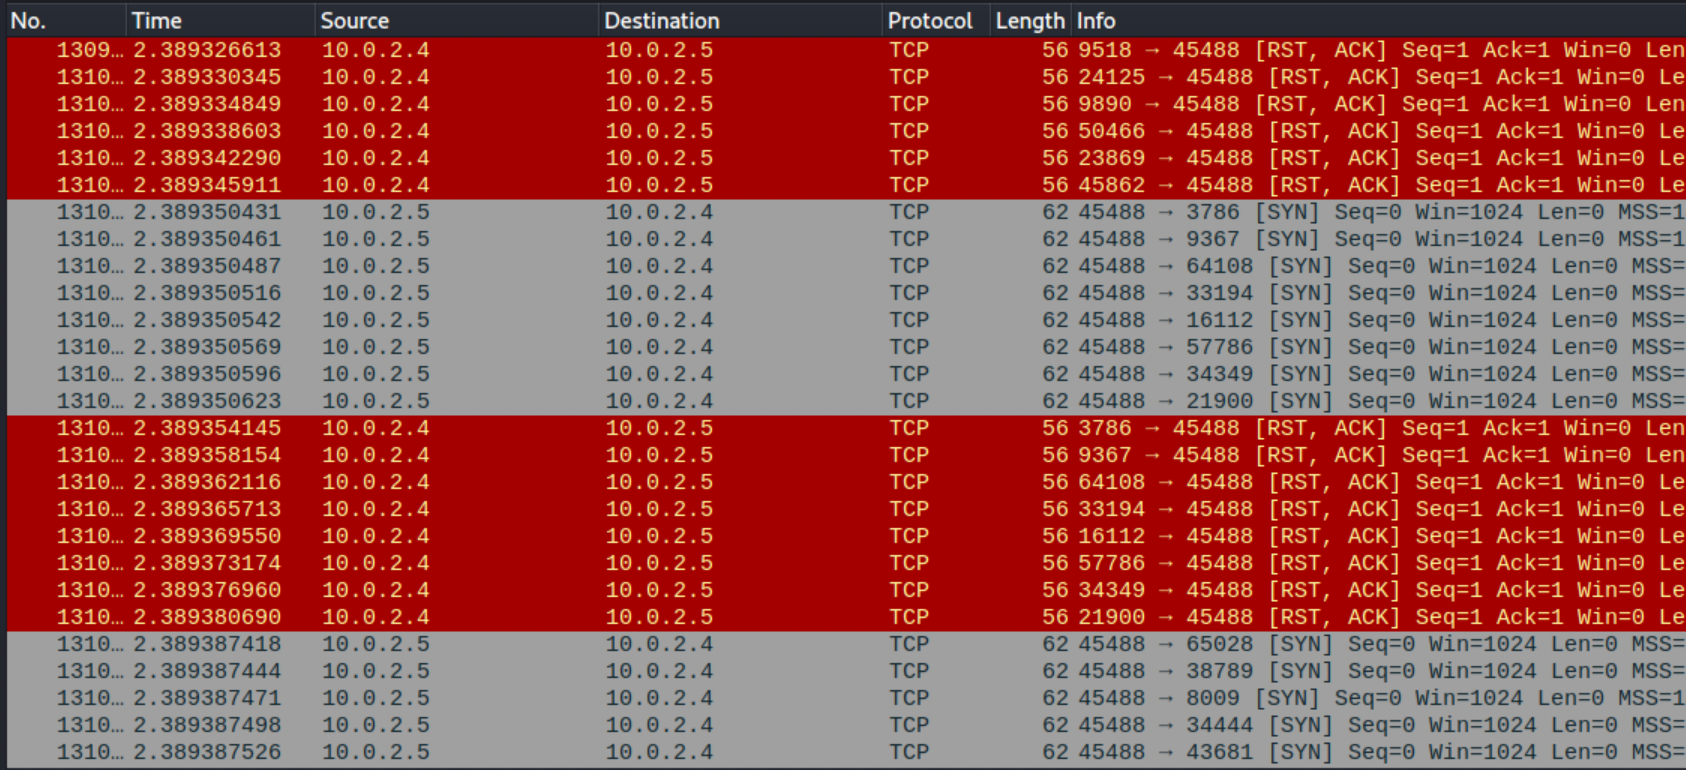
\includegraphics[width=\linewidth]{img/ws_firewall-open.png}
	\caption{Datenverkehr bei offener Firewall}
	\label{fig:ws_firewall_open}
\end{figure}

Im Wireshark-Mitschnitt (Abbildung \ref{fig:ws_firewall_open}) wird der Datenverkehr der Opfermaschine gezeigt. Zu erkennen in grau, sind die eingehenden Anfragen der Angreifermaschiene. Hier werden TCP SYN Anfragen an das Opfer geschickt und eine ACK bzw. RST Antwort erwartet. Dies ist die Einleitung einer TCP Verbindung, welche bei diesem Scan nie vollständig durchgeführt wird. Da die Ports der Opfermaschine nicht gefiltert werden, werden die Anfragen verarbeitet und dem Angreifer wird geantwortet. Bei Eingang einer ACK oder RST Nachricht auf der Angreifermaschiene wird der Kontakt zum Port abgebrochen und somit keine Verbindung erstellt. Alleine durch das Antworten verrät das Opfer bereits den Status der Ports. Sollte der Angreifer eine ACK Nachricht erhalten, so ist der gefragte Port offen und "hört" auf einkommende Anfragen. Im Falle einer RST Nachricht ist der Port geschlossen.
 Sollte keine Antwort verschickt werden interpretiert NMAP den Port als gefiltert. Ein SYN Scan eignet sich besonders aufgrund der Geschwindigkeit des Scans und der Verlässlichkeit der Ergebnisse.

\subsubsection{nmap 10.0.2.4 -sU -T4}
 Zu prüfen, ob die Verbindung via UDP ebenfalls offen ist, wird als nächster Schritt ein UDP Scan mit NMAP durchgeführt. Wie bei dem vorherigen Scan sind hier ebenfalls die Parameter für die Geschwindigkeit gesetzt. Der -A Parameter wurde gegen -sU ausgetauscht. Der -sU Parameter gibt den Scantyp an. So wird anstatt eines TCP SYN Scans ein UDP Scan durchgeführt. Obwohl TCP den Großteil des Internetverkehrs prägt, ist UDP kein zu vernachlässigendes Protokoll. Bei diesem Scan werden UDP Pakete an die Ports geschickt. NMAP erwartet im Gegenzug ICMP Antworten. Entweder die Opfermaschine schickt eine Nachricht, dass der gewünschte Port nicht erreichbar ist – Port ist geschlossen – oder es wird eine andere Errornachricht verschickt, in welchem Falle der Port als gefiltert gesehen wird. Sollte das Opfer eine UDP Antwort verschicken, so ist der Port offen. Sei es der Fall, dass der Angreifer keine Antwort erhält wird der Port als entweder offen oder gefiltert interpretiert. 
Ein großes Hindernis an UDP Scanning ist der Zeitaufwand, da NMAP bei offenen Ports keine Antwort erhält und daraufhin auf den Timeout warten muss. Auf Grund dessen werden bei diesem Scan nur die wichtigsten 1000 Ports gescannt. Zudem ist die Verbindung via UDP wesentlich unverlässlicher als über TCP, was zu verfälschten Ergebnissen führen kann.

\begin{figure}
	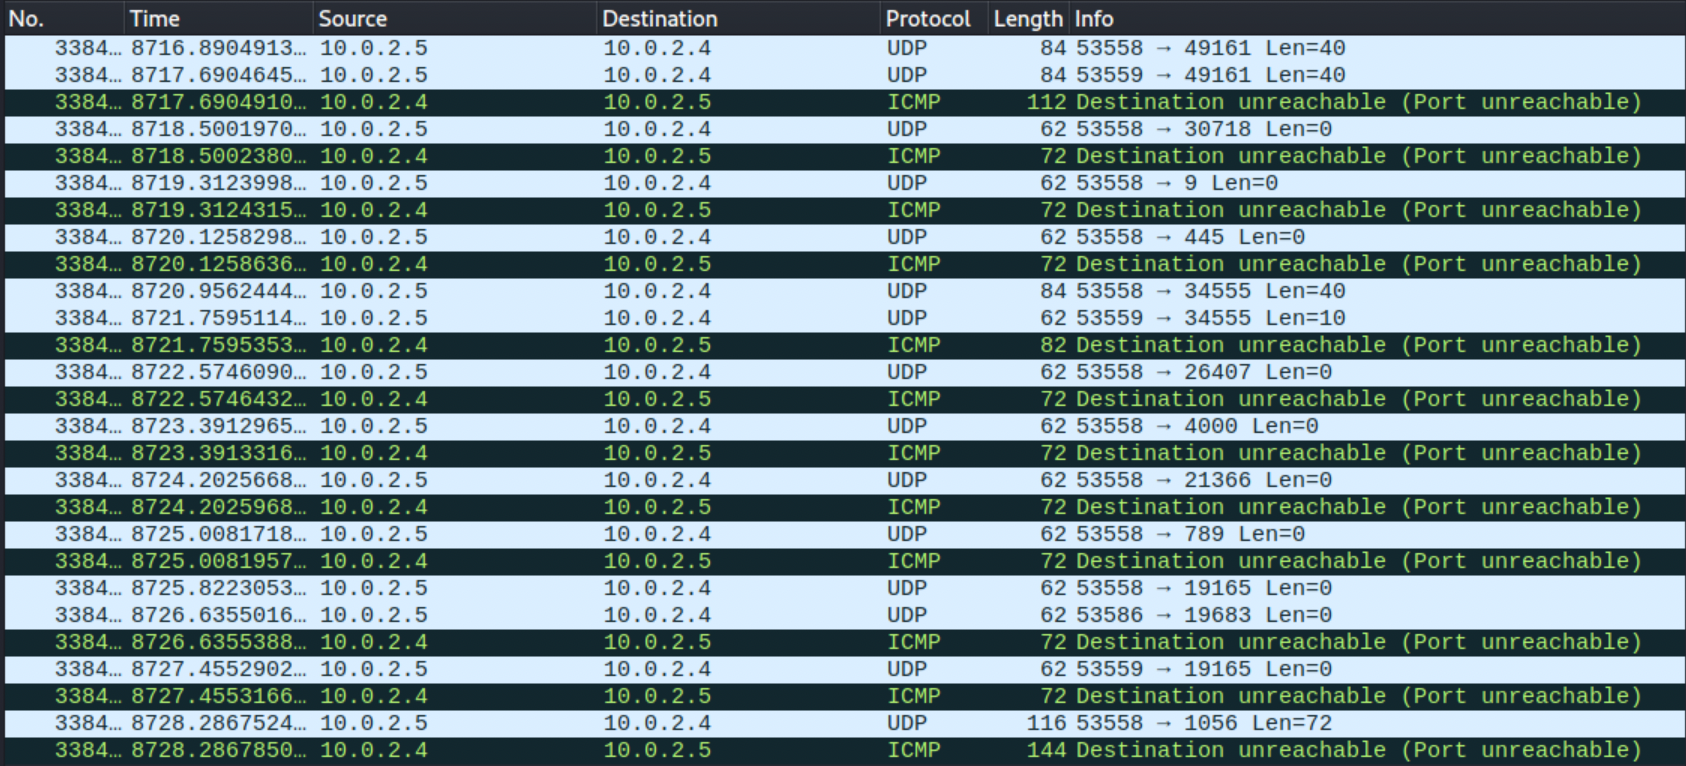
\includegraphics[width=\linewidth]{img/ws_firewall_open_udp.png}
	\caption{Datenverkehr bei offener Firewall – UDP}
	\label{fig:ws_firewall_open_udp}
\end{figure}

Auf der Abbildung \ref{fig:ws_firewall_open_udp} ist zu erkennen, wie der UDP Scan verläuft. Wie bereits beschrieben werden der Opfermaschine UDP Pakete geschickt (zu sehen in Blau). Darauf folgt die Antwort des Opfers – in diesem Fall als ICMP Error – dass der gewünschte Port nicht zu erreichen ist. Aus diesem Grund interpretiert NMAP die Ports der Opfermaschine als geschlossen. \newpage

\lstinputlisting{scripts/scans/nmap_sU_T4}

Am Output des Scans lässt sich erkennen, dass dieser wesentlich länger gebraucht hat als der vorherige TCP Scan. So hat der UDP Scan 18 Minuten gebraucht um die wichtigesten 1000 Ports des Opfers zu scannen. Desweiteren wird berichtet, dass acht Ports offen bzw. gefiltert sind. Da keine Services auf der Opfermaschine laufen oder Firewall-Filter gesetzt sind lässt sich vermuten, dass diese Ports fehlerhaft als offen | gefiltert angezeigt werden. So kann es sein, dass die Opfermaschine nicht schnell genug auf die Anfragen des Angreifers geantwortet haben und somit der Timeout von NMAP erreicht wurde. 

\subsection{Penetrationtest - Outward}

\section{Geschlossene Konfiguration}
Als nächstes wird eine Konfiguration getestet, in der alle Verbindungen geblockt werden. Zu dieser Konfiguration gehören die Ausnahmen: SSH und localhost. Das Ziel dieses Tests ist es zu prüfen, wie die Opfermaschine von außen angesprochen werden kann – bzw. welche Informationen ein potentieller Angreifer erhalten könnte.
 
\subsection{Script}
Dieses Script besteht aus sechs Teilen: 
\begin{itemize}
	\item Flushing der Regeln
	\item Ausnahmeregelungen
	\item Standardregelungen
	\item Localhost
	\item Bestehende Verbindungen
	\item Logging
\end{itemize}
Zunächst werden alle bestehenden Regeln gelöscht. Dies geschieht wie in dem vorherigen Script mit Hilfe des Flushingbefehls. Darauf folgen die Ausnahmeregelungen. Diese werden hier als nächstes gesetzt, da die Reihenfolge der Regeln bei den IP-Tables durchaus einen Einfluss hat. In diesem Fall wird der Port 22 freigegeben. Sowohl eintreffende wie auch ausgehende Nachrichten dürfen über den Port 22 gehandhabt werden. Dies erlaubt es mit der Virtual Machine eine SSH Verbindung aufzubauen. \\
Um dann die Firewall so einzustellen, dass keine weiteren Verbindungen zugelassen werden, werden nun die Standardregelungen gesetzt. Im Gegenzug zum vorherigen Script werden nun die eingehenden, ausgehenden und weitergeleiteten Verbindungen "gedroppt". So werden alle Pakete die über die betroffenen Ports laufen fallen gelassen und nicht bearbeitet. \\
Damit trotzdessen der localhost weiterhin funktioniert, werden noch einmal Ausnahmen beschrieben.
Zusätzlich werden bestehende Verbindungen weiterhin zugelassen, um keine laufenden Prozesse zu stören. Somit kann gesichert sein, dass plötzliche Änderungen in der Firewall keine Probleme in der Anwendung mitsichziehen. 
Abschließend werden erneut die Loggingbefehle gesetzt.

\newpage

\lstinputlisting[language=bash]{scripts/firewall-closed.sh}

\newpage

\lstinputlisting{scripts/output_firewall-closed}

\subsection{Penetrationtest – Inward}
Nun sind alle Ports der Opfermaschine geblockt bzw. gefiltert. Um zu überprüfen, ob das Script funktioniert hat werden nun eine Reihe an Tests abgeschlossen. Zunächst werden wieder NMAP Scans die Grundlage bilden, von der wichtige Informationen über das Ziel abgeleitet werden können.

\subsubsection{nmap 10.0.2.4 -p- -A -T4}
Es wird nun erneut mittels eines TCP SYN Scans geprüft, welche Ports des Opfers offen sind. Zu Gunsten der Genauigkeit und der Vergleichbarkeit des Scans wurde die Konfiguration der Parameter aus dem Kapitel 2.1.2 übernommen.
Ebenfalls wird erneut der Datenverkehr der Opfermaschine aufgezeichnet. 
\newpage
\lstinputlisting{scripts/scans/nmap_p_A_T4_closed}

An der Ausgabe des Scans lässt sich erkennen, dass trotz der verschärften Regelungen die MAC Adresse sowie der Hersteller des Geräts erkannt wurde. 
Der wichtigste Punkt ist jedoch, dass alle Ports des Opfers nun als gefiltert anstatt als geschlossen erkannt werden. Dies liegt daran, dass keine Antwort auf die SYN Pakete des Angreifers verschickt werden. Wie bereits beschrieben, interpretiert NMAP bei einem TCP SYN Scan das Fehlen einer Antwort als Filterung des angesprochenen Ports. Dies wird anhand der Abbildung \ref{fig:ws_firewall_closed} deutlich. Dort ist zu sehen, wie die Pakete der Angreifermaschiene von der Adresse 10.0.2.5 auf der Opfermaschine eintreffen. Jedoch antwortet die Opfermaschine nicht, anders als in Abbildung \ref{fig:ws_firewall_open}.

\begin{figure}
	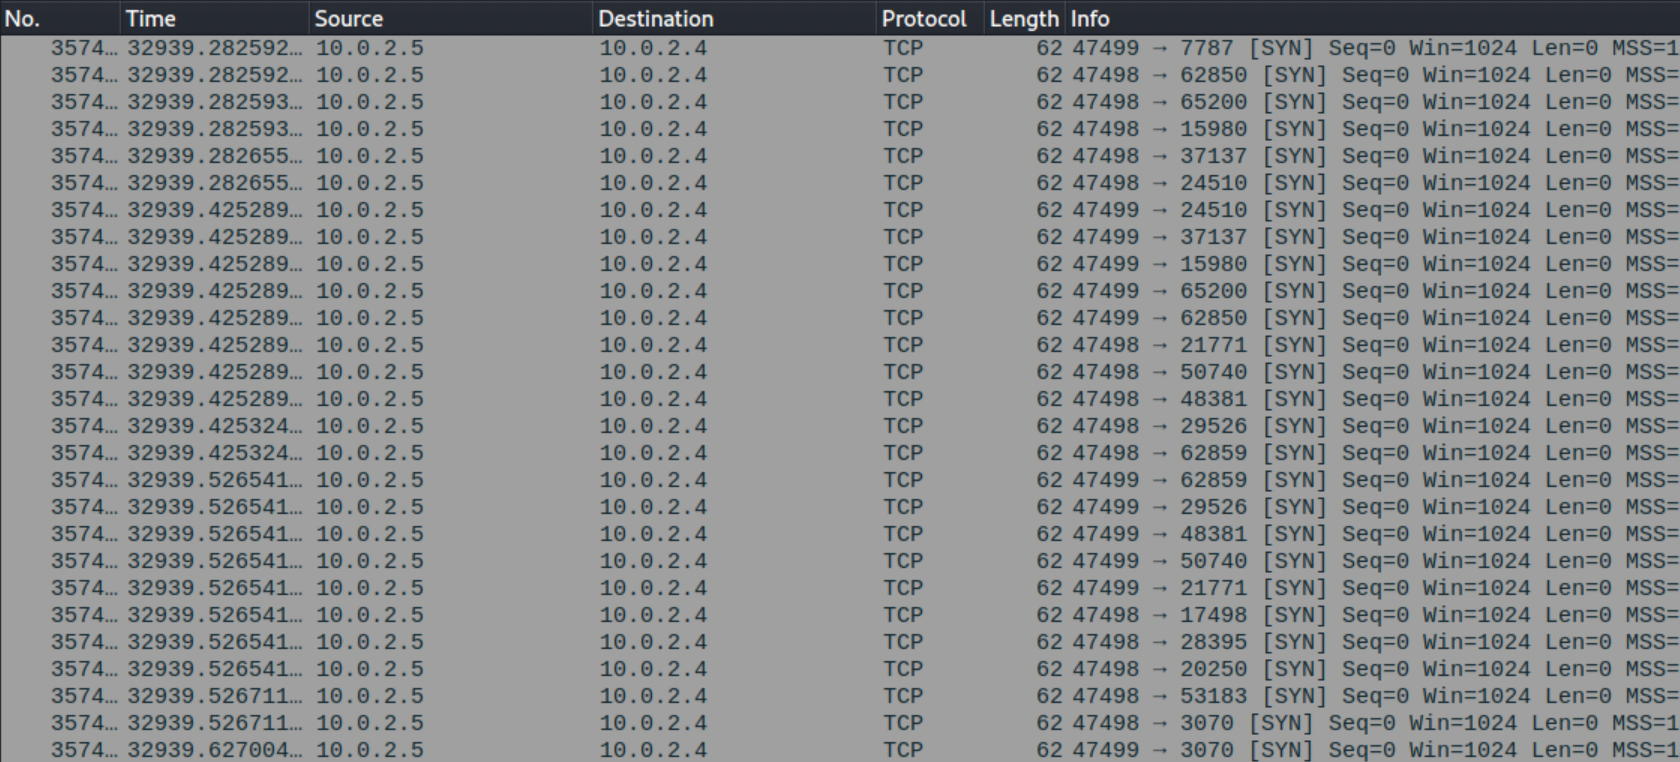
\includegraphics[width=\linewidth]{img/ws_firewall_closed.png}
	\caption{Datenverkehr bei geschlossener Firewall}
	\label{fig:ws_firewall_closed}
\end{figure}

\subsubsection{nmap 10.0.2.4 -sU -T4}
Um zu Prüfen, welchen Einfluss das Script auf UDP Pakete nimmt, wird als nächstes ein UDP Scan durchgeführt. Wie auch beim vorherigen Scan, bleiben die Parameter gleich. Die Erwartung an dieses Scanergebnis ist, dass alle Ports der Opfermaschine als offen | gefiltert angezeigt werden. Zudem wird erwartet, dass dieser Scan wesentlich mehr Zeit in Anspruch nimmt, als der Scan aus dem Kapitel 2.1.2. Diese Erwartungshaltung bildet sich aus der Art und Weise, wie der UDP Scan funktioniert. Da die Ports des Opfers durch das Bash-Script geschlossen sein sollten, sollten keine Antwortpakete an den Angreifer geschickt werden. Somit müsste der Angreifer auf den Timeout von NMAP warten, welcher zur gleichen Zeit die Ports als offen bzw. gefiltert interpretiert.

\begin{figure}
	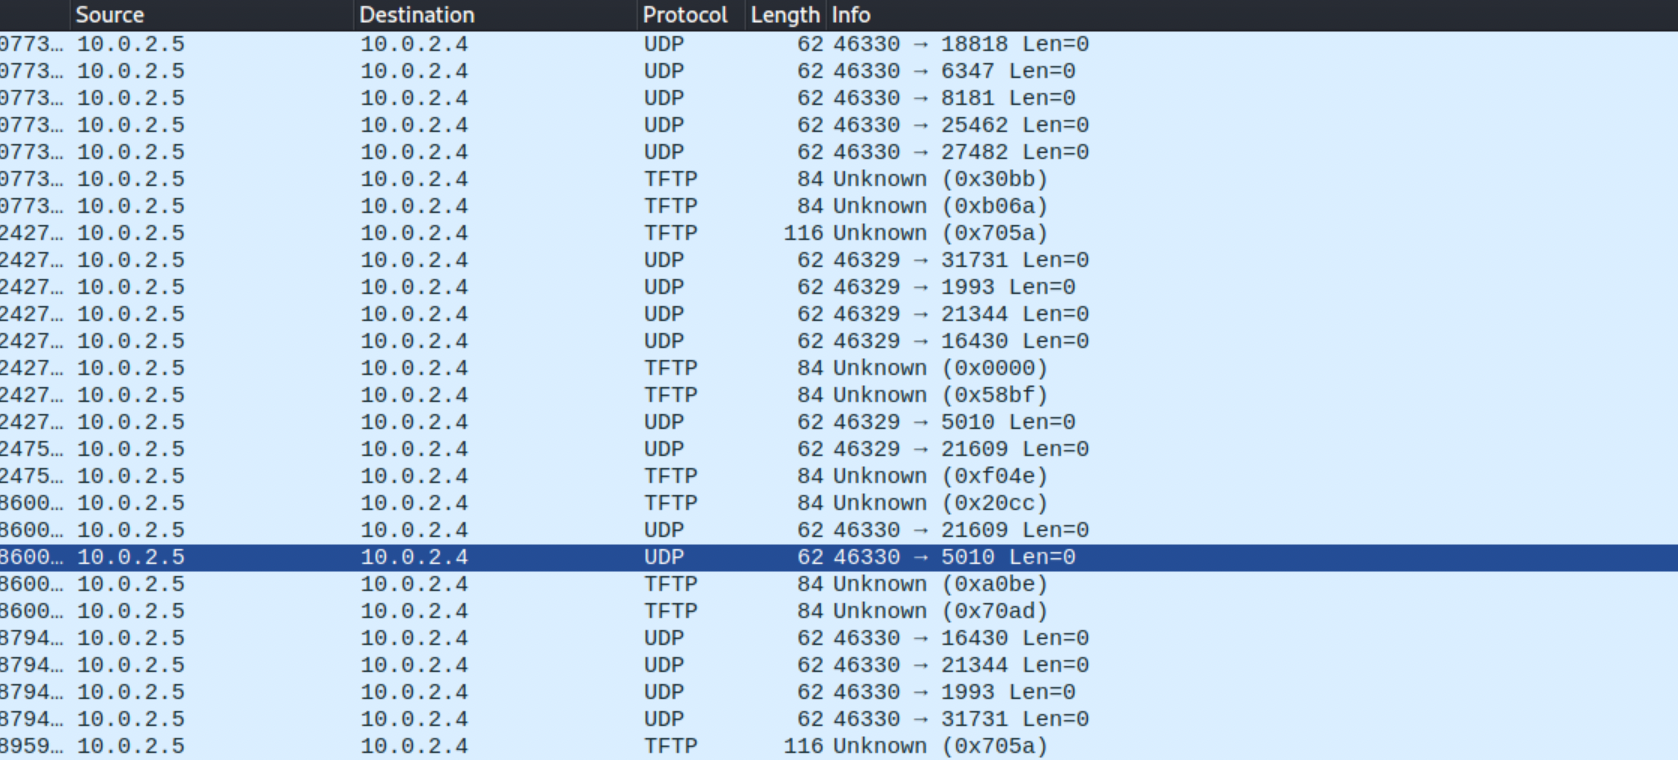
\includegraphics[width=\linewidth]{img/ws_firewall_closed_udp.png}
	\caption{Datenverkehr bei geschlossener Firewall – UDP}
	\label{fig:ws_firewall_closed_udp}
\end{figure}
Output:
\lstinputlisting{scripts/scans/nmap_sU_T4_closed}

Der Output bestätigt die Hypothese. Da der Angreifer keine Antworten erhalten hat, kann keine genaue Aussage über den Status der Ports getroffen werden. 

\subsection{Penetrationtest – Outward}
Lorem ipsum dolor sit amet, consectetur adipiscing elit. Vestibulum fermentum semper mollis. Ut porta odio in ultrices fermentum. Aenean id pulvinar nisi. Phasellus porttitor condimentum suscipit. Nulla facilisi. Mauris in malesuada arcu. Morbi tempus bibendum tempor.

Vivamus sit amet tellus pellentesque, commodo est vitae, interdum ante. In eu vestibulum dolor, in venenatis felis. Ut risus odio, convallis in aliquet quis, luctus quis sem. Vivamus malesuada ex eget vehicula finibus. Mauris iaculis finibus diam vel ultrices. Morbi luctus nulla euismod sodales posuere. Integer dignissim gravida orci, at porttitor nibh varius ac. Donec vel efficitur nulla. In fermentum mauris elit, a efficitur elit accumsan id. Interdum et malesuada fames ac ante ipsum primis in faucibus.

Proin lacinia malesuada leo sit amet bibendum. Integer dictum ultrices enim id condimentum. Ut egestas vulputate quam. Pellentesque bibendum nec turpis ac ultricies. Sed at ligula nec urna bibendum convallis consequat at turpis. Sed id dolor eros. Nullam maximus turpis in massa ornare accumsan. Sed id dapibus eros, tincidunt ullamcorper risus. In tincidunt, nunc at suscipit placerat, nulla justo imperdiet est, id convallis libero elit a nulla. Vivamus velit odio, convallis sed dignissim vitae, pharetra eu tellus. Sed eu dignissim felis, ac rhoncus est. Vivamus ac aliquam urna. Pellentesque lectus risus, porta eu diam in, volutpat pharetra justo. Donec elit diam, maximus vitae congue et, condimentum a magna. 

\newpage
\section{Standard Konfiguration}

\lstinputlisting[language=bash]{scripts/firewall-standard.sh}

\subsection{Script}
Das Script zur Erstellung einer Firewall, wie sie möglicherweise in Unternehmen vorkommen könnte, ähnelt dem aus Kapitel 2.2.1 sehr. 
Es besteht aus den gleichen sechs Teilen, obwohl das Logging hier auf Grund der Länge des Scripts vernachlässigt wird.
Zunächst werden alle bestehenden Regeln gelöscht – gefluscht – um die Firewall auf ihre Basiskonfiguration zurückzusetzen. Dies verhindert mögliche Konflikte mit bestehenden Regeln im weiteren Verlauf. 

\subsection{Penetrationstest – Inward}
Lorem ipsum dolor sit amet, consectetur adipiscing elit. Vestibulum fermentum semper mollis. Ut porta odio in ultrices fermentum. Aenean id pulvinar nisi. Phasellus porttitor condimentum suscipit. Nulla facilisi. Mauris in malesuada arcu. Morbi tempus bibendum tempor.

Vivamus sit amet tellus pellentesque, commodo est vitae, interdum ante. In eu vestibulum dolor, in venenatis felis. Ut risus odio, convallis in aliquet quis, luctus quis sem. Vivamus malesuada ex eget vehicula finibus. Mauris iaculis finibus diam vel ultrices. Morbi luctus nulla euismod sodales posuere. Integer dignissim gravida orci, at porttitor nibh varius ac. Donec vel efficitur nulla. In fermentum mauris elit, a efficitur elit accumsan id. Interdum et malesuada fames ac ante ipsum primis in faucibus.

Proin lacinia malesuada leo sit amet bibendum. Integer dictum ultrices enim id condimentum. Ut egestas vulputate quam. Pellentesque bibendum nec turpis ac ultricies. Sed at ligula nec urna bibendum convallis consequat at turpis. Sed id dolor eros. Nullam maximus turpis in massa ornare accumsan. Sed id dapibus eros, tincidunt ullamcorper risus. In tincidunt, nunc at suscipit placerat, nulla justo imperdiet est, id convallis libero elit a nulla. Vivamus velit odio, convallis sed dignissim vitae, pharetra eu tellus. Sed eu dignissim felis, ac rhoncus est. Vivamus ac aliquam urna. Pellentesque lectus risus, porta eu diam in, volutpat pharetra justo. Donec elit diam, maximus vitae congue et, condimentum a magna.
\subsection{Penetrationtest – Outward}

Lorem ipsum dolor sit amet, consectetur adipiscing elit. Vestibulum fermentum semper mollis. Ut porta odio in ultrices fermentum. Aenean id pulvinar nisi. Phasellus porttitor condimentum suscipit. Nulla facilisi. Mauris in malesuada arcu. Morbi tempus bibendum tempor.

Vivamus sit amet tellus pellentesque, commodo est vitae, interdum ante. In eu vestibulum dolor, in venenatis felis. Ut risus odio, convallis in aliquet quis, luctus quis sem. Vivamus malesuada ex eget vehicula finibus. Mauris iaculis finibus diam vel ultrices. Morbi luctus nulla euismod sodales posuere. Integer dignissim gravida orci, at porttitor nibh varius ac. Donec vel efficitur nulla. In fermentum mauris elit, a efficitur elit accumsan id. Interdum et malesuada fames ac ante ipsum primis in faucibus.

Proin lacinia malesuada leo sit amet bibendum. Integer dictum ultrices enim id condimentum. Ut egestas vulputate quam. Pellentesque bibendum nec turpis ac ultricies. Sed at ligula nec urna bibendum convallis consequat at turpis. Sed id dolor eros. Nullam maximus turpis in massa ornare accumsan. Sed id dapibus eros, tincidunt ullamcorper risus. In tincidunt, nunc at suscipit placerat, nulla justo imperdiet est, id convallis libero elit a nulla. Vivamus velit odio, convallis sed dignissim vitae, pharetra eu tellus. Sed eu dignissim felis, ac rhoncus est. Vivamus ac aliquam urna. Pellentesque lectus risus, porta eu diam in, volutpat pharetra justo. Donec elit diam, maximus vitae congue et, condimentum a magna.

\chapter{Projektphase 2 – Webserver}
\section{Setup}
\subsection{Datenbank}
Für das Projekt wurde PostgreSQL (auch Postgres) als Datenbank gewählt. So wurde über Docker eine Container-Instanz einer Postgres Datenbank gestartet, die auf dem localhost der Hostmaschine läuft. \\
Die Datenbank enthält zwei Tabllen – User und Post – welche jeweils eine inkrementierende ID als Primärschlüssel besitzen. 
Die Tabelle User enthält dabei zusätzlich den Benutzernamen und das Passwort des Nutzers – wobei beide bewussterweise im Klartext gespeichert werden. 
Die Tabelle Post enthält neben der ID noch die Attribute Title und Content, welche bei der Ausgabe der Posts angezeigt werden. 
\subsection{API}
Zur Demostration der beiden Attacken werden zwei APIs genutzt. Beide werden mit Hilfe des Express.js Frameworks implementiert. \\
Die erste – und umfangreichere – API stellt die Schnittstelle zur Datenbank der Blog-Applikation dar. Hier werden die typischen CRUD Operationen durchgeführt und ans Frontend angebunden. Zudem wird ein Teil der Sessionerstellung hier geregelt. \\
Die andere API stellt den Angreifer dar. Sie bietet auch nur eine Schnittstelle, über welche der Session-Cookie des Opfers gesendet wird. 
\subsection{Frontend}
Das Frontend bildet einen Webblog ab, welcher das Posten von Textbeiträgen ermöglicht. So wie in der Datenbank abgebildet, werden hier Titel und Content eingetragen und an die API verschickt. \\
Das Frontend wurde mit Vue.js entwickelt und bietet aus diesem Grund einige prädefinierten Sicherheitsfunktionen, die eine \ac{XSS}-Attacke vorbeugen sollen. 
Aus diesem Grund werden die Inhalte aus der Datenbank mit Hilfe des v-HTML Attributs in das Frontend eingebunden, anstatt der üblichen ``Mustache`` Notation.
\section{Cross-Site-Scripting}

Unter dem Begriff \ac{XSS} versteht man einen Typ der Injektionsattacken, bei dem schadhafter Code – oft in Form eines browserseitigen Scripts – bei einem Endnutzer ausgeführt wird. Diese werden durch mangelhafte bzw. fehlende Überprüfung von Nutzereingaben ermöglicht. \\
Um dieses zu demonstrieren, wurde bei diesem Projekt bewusst darauf verzichtet Nutzereingaben zu überprüfen. 

Das Ziel der Demonstration ist es den Session-Cookie zu stehlen. Um dies zu erreichen wird ein neuer Blog-Post erstellt, wo anstatt eines Textes ein fehlerhaftes HTML <img> Element eingegeben wird. Beim erneuten Aufrufen der Seite wird nun von der Anwendung versucht ein Bild für dieses <img> zu rendern, erhält jedoch nur einen Fehler, da die URL bewusstermaßen fehlerhaft ist. 
Nun ist es möglich mittels des HTML Attributs "onerror" der Applikation vorzuschreiben, wie mit dem Fehler umzugehen ist. Dies wird mittels validem JavaScript Code geschafft. So wird nun ein Request an die hostile API gesendet, wo über die document.cookie funktion nun der Session-Cookie übertragen wird. 
Abschließend ist der Session-Cookie auf der Console des hostilen Servers zu finden.

\section{SQL Injection}